%*****************************************
\chapter{Experiments}\label{ch:experiments}
%*****************************************

\section{Blocks World as a Simple Real-Time Symbolic Control Problem Domain}

\begin{figure}[bth]
  \center
  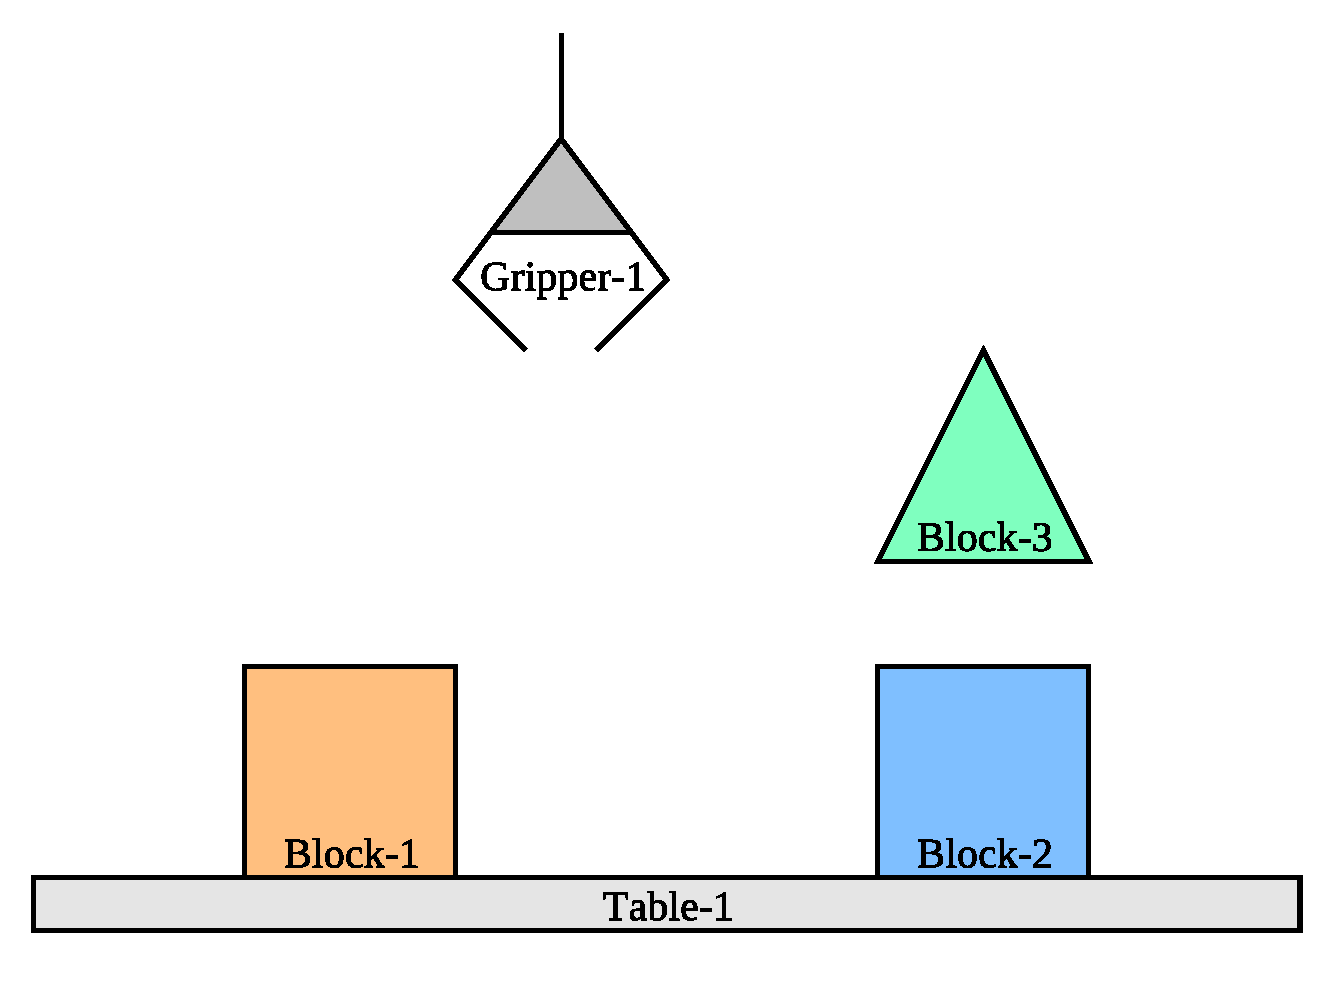
\includegraphics[width=11cm]{gfx/blocks_world_screenshot-1}
  \caption[Blocks world is a simple real-time symbolic control problem]{Blocks world is a simple real-time symbolic control problem that I use to demonstrate my reflective control learning theory.}
  \label{fig:blocks_world_screenshot-1}
\end{figure}

I use blocks world, a canonical toy AI problem, in order to demonstrate my example of reflectively learning to plan.
See Figure~\ref{fig:blocks_world_screenshot-1} for a screenshot of my blocks world problem physical simulation.

\begin{table}
  \myfloatalign
  \begin{tabularx}{\textwidth}{XllX}
    & [Gripper-1 is me] & [Gripper-1 movement\_command []] & \\
    & [Gripper-1 is-a gripper] & [Gripper-1 color black] & \\
    & [Gripper-1 is-holding []] & [Block-1 is-a block] & \\
    & [Block-1 color brown] & [Block-1 shape cube] & \\
    & [Block-1 on Table-1] & [Block-1 left-of Gripper-1] & \\
    & [Block-2 is-a block] & [Block-2 color blue] & \\
    & [Block-2 shape cube] & [Block-2 on Table-1] & \\
    & [Block-2 right-of Gripper-1] & [Block-3 is-a block] & \\
    & [Block-3 color green] & [Block-3 shape pyramid] & \\
    & [Block-3 right-of Gripper-1] & [Table-1 is-a block] & \\
    & [Table-1 color white] & [Table-1 shape cube] & \\
    & [Table-1 left-of Gripper-1] & &
  \end{tabularx}
  \caption[Blocks world AI perceptual input]{Blocks world AI perceptual input.}
  \label{tab:blocks_world_agent_perceptions}
\end{table}

See Table~\ref{tab:blocks_world_agent_perceptions} for an example set of perceptual input that corresponds with the physical situation shown in Figure~\ref{fig:blocks_world_screenshot-1}.

\section{A Concrete Plan}


%Feedback from Committee:
%
%  Needed by Wednesday:
%
%    -- A plan that says what I'll do.
%    -- What tests I will run and how I intend to interpret the results.
%    -- Preferably: A revised outline of the thesis.
%
%    For the Implementation:
%
%      -- Show dense reflective traceback.
%
%        -- For example, I need to show the traceback working when the
%           system encounters a realistic bug.
%
%        -- I should also show how this traceback data would be used to
%           revise execution.
%
%    For the Thesis:
%
%      -- Make the thesis clear in the document from the outset, and
%         stick to these ideas throughout.
%
%MY ADVICE IS TO DEVELOP A SIMPLE AND CLEAR NARRATIVE RUNNING FROM YOUR CONTRIBUTIONS TO YOUR IMPLEMENTATION THROUGH YOUR THEORY. YOU START VERY SIMPLE AND DEVELOP IT BY ADDING TECHNICAL DETAIL AS YOU PROCEED. TO DO THIS, IT IS IMPORTANT TO DETERMINE WHAT YOU WILL *NOT* SAY AS MUCH AS WHAT YOU WILL SAY. 
%
%        -- Use the defense material for focus.
%
%        -- Make clear what has been implemented.
%

\subsection{Credit Assignment Metric}

  First, I will develop a metric by which I can measure the
  performance of my credit assignment algorithm versus other
  algorithms.  At one extreme, we have the brute force approach to
  learning, in which all possible concepts are re-learned at every
  opportunity (e.g. at every step in a Markov stepped system, or at
  every knowledge event in my real-time event driven system).  At the
  other extreme, we re-learn only those concepts whose fundamental
  training knowledge has changed (instances, hypothesis space, or
  features).  My approach to tracing the provenance of deliberative
  knowledge through the reactive plan execution agencies will be
  somewhere between these two extremes of efficiency.


  -- Evaluation Metrics

     -- credit assignment: the process of choosing a subset from the
                           total possible set of concepts that should
                           be focused on as being responsible for the
                           occurrence of a given event.

EXACTLY WHAT IS THE METRIC HERE? HOW WILL IT BE MEASURED? YOU HINT AT SPEED BELOW, AND IF THIS IS TRUE, WILL IT BE MEASURED IN DECISION-CYCLE TIME? DEFINE AND OPERATIONALIZE YOUR METRIC.

       The credit assignment process can be more or less efficient in
       focusing the learning resources toward concepts that can be
       re-learned.

\subsection{Temporal Credit Assignment}

       I can measure the performance of my causal credit assignment
       algorithm versus a typical temporal credit assignment
       algorithm, such as an adaptation of the Temporal Difference
       (TD) learning algorithm commonly used in the field of
       reinforcement learning.

HAVE YOU ALREADY IMPLEMENTED THIS ALGORITHM? WILL YOU USE AN EXISTING IMPLEMENTATION?

\subsection{Causal Credit Assignment}

        The goal of these tests are to show that learning by
        provenance speeds the standard temporal credit assignment
        method, which assigns credit to the sequence of immediately
        previous states and actions.

ABOVE YOU MENTION YOUR CREDIT ASSIGNMENT *VERSUS* A STANDARD ALGORITHM. HERE YOU STATE THAT YOUR VERSION WILL ACCELERATE THE STANDARD ALGORITHM. DO YOU MEAN THAT YOURS IS FASTER THAT THE STANDARD IN THE LIMIT? OR DO YOU INTEND TO COMBINE THEM TO SPEED UP THE TEMPORAL ALGORITHM? 

     -- I will focus on re-learning category concepts given new
        training instances that would change those concepts.

  -- Now, given the above metric for what I will actually be measuring
     as a performance metric, here are two specific deliberative
     learning tasks where my causal learning will be superior to a
     temporal credit assignment method.  This is primarily due to the
     delayed time between deliberation about knowledge and the
     execution of that knowledge, resulting in a precondition check
     form of failure.  Specifically, the precondition check could
     simply be what would be Removed by a trans-frame, but doesn't
     necessarily exist in the physical knowledge at the time of
     execution.  The following are two examples of scenarios:

\subsection{The Social Knowledge Trust Task}

        Some plans can be learned through a social communication
        language.  Physical plans are added to the deliberative
        knowledge with the added relationship with the appropriate
        social provenance markers, e.g. Gripper-1 may represent that a
        given plan is told to it by The-User (or another social
        source).

        The Decision to use a plan that accomplishes a given goal from
        one knowledge source or another can be learned, but the
        learning of this type of action is difficult because of the
        often indirect temporal connection between this deliberative
        Decision involved in choosing or creating a plan and the
        actual execution failure, resulting from executing a plan that
        has derived from that deliberative decision.

THIS LONG RUN-ON SENTENCE IS TYPICAL OF YOUR WRITING AND PLACES THE BURDEN OF UNDERSTANDING UPON THE READER. WHAT IS LEARNED? A DECISION OR AN ACTION? FURTHERMORE, YOU PREVIOUSLY DISCUSSED LEARNING CONCEPTS. IMPLEMENT A SINGLE LEARNING ALGORITHM AND USE IT TO ILLUSTRATE YOUR THEORY. AGAIN, DECIDE WHAT YOU WILL NOT SAY.


\subsection{Working in a World of Building Blocks}

In his PhD thesis, Terry Winograd worked in the world of building
blocks \citep{winograd:1970}.  This program maintained traces of its
goals and subgoals, which enabled it to answer questions about why it
performed certain actions.  This system worked because it stored
goals.

Knowing the goal state of the computation is important, and I do not
ignore this aspect in tracing the deliberative layer.  My system is
able to answer these sorts of questions, as this simply requires
climbing the stack of mental resource activations, but when debugging
the deliberative process, it is helpful to not only know the ending
point of computation but also the means toward that end.

\subsection{Terry Winograd's SHRDLU and Goal Tracing}

I am building upon what was learned from Winograd's thesis
\citep{winograd:1970} in terms of using traces of the deliberative
process as well as using a semantic model of the world in order to
understand communications between AIs.  I have chosen to use a
simpler and more direct language interface between AIs that refers
more directly to the semantic information and mental processes
involved.  I have experimented with implementing the original SHRDLU
english language parser, although I believe the parsing process can be
better controlled as a goal-oriented set of concurrent processes than
as the stack-based depth first search that I started writing in my
initial experiments.


\section{A Physical Simulation of a Kitchen as a Social Commonsense Reasoning Domain}

\begin{figure}[bth]
  \center
  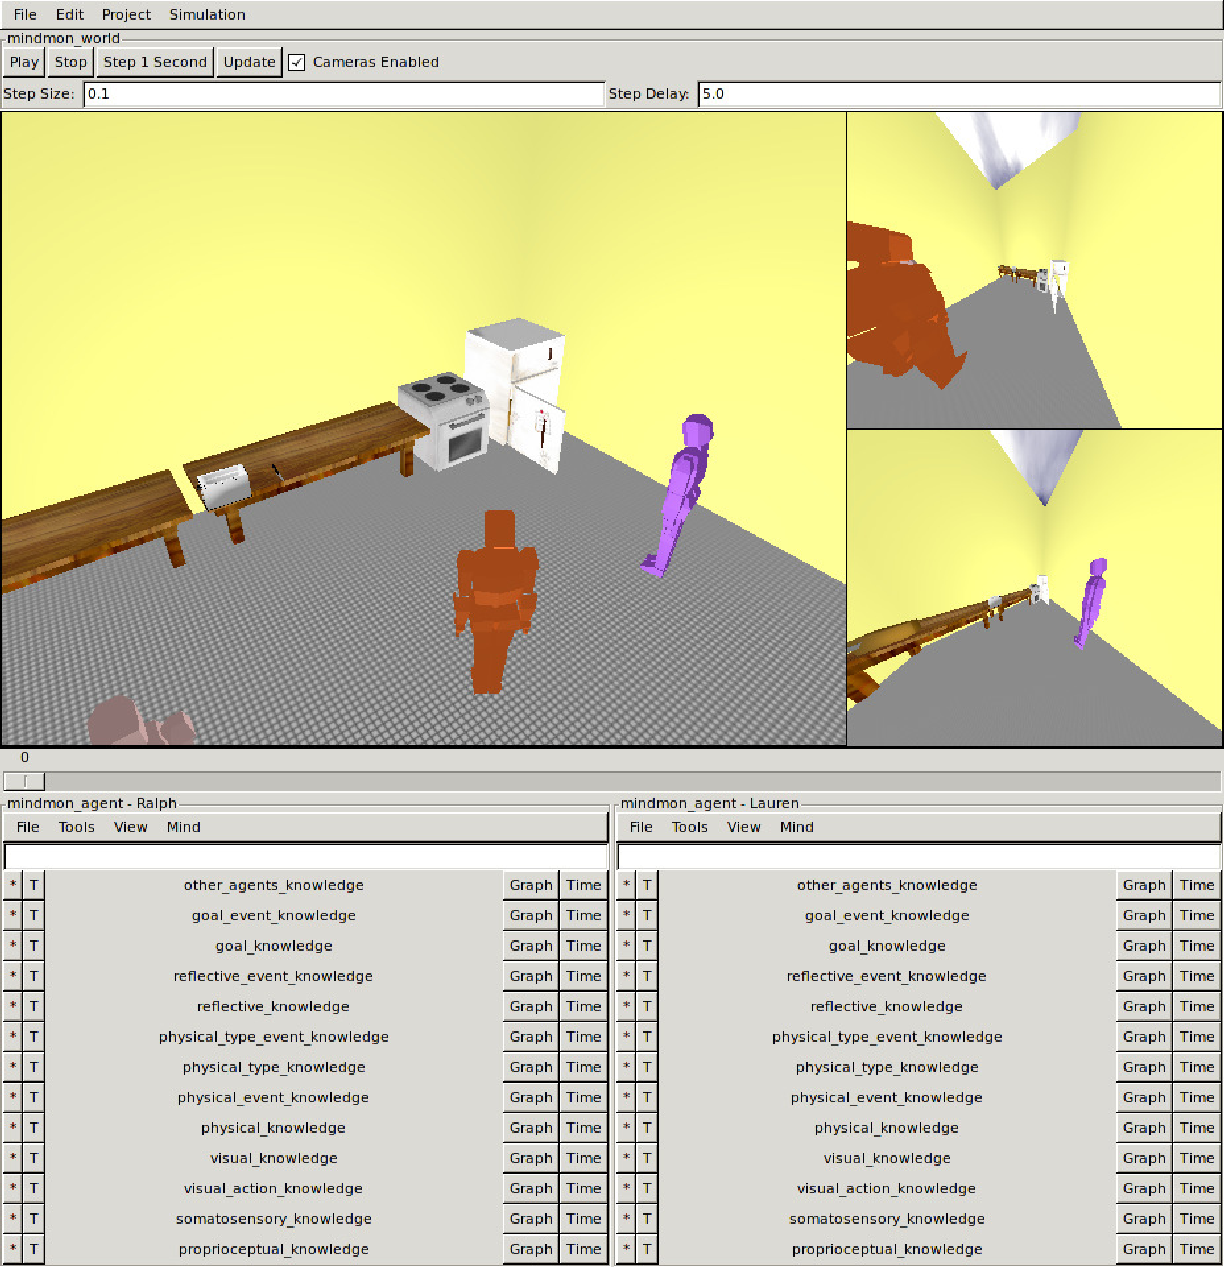
\includegraphics[width=11cm]{gfx/mindmon-isis_world-screenshot-1}
  \caption[Isis World is a larger physical simulation than the Blocks
    World toy problem]{Isis World is a larger real-time symbolic
    physical simulation, which I use to demonstrate that my reflective
    goal-oriented learning approach scales to the physical and
    reflective problem spaces of slightly more complicated learning
    problems.}
  \label{fig:mindmon-isis_world-screenshot-1}
\end{figure}

I have experimented with applying my cognitive architecture to a
larger social commonsense reasoning domain with parents that teach
children as they attempt to accomplish cooking tasks in a kitchen.
See \cite{morgan:2011} for details about my six-layered reflective
theory of social and moral reasoning, which assumes the existence of a
procedurally reflective infrastructure with a reflective problem
solver written within it.

\subsection{Why Not Work Solely Within the Blocks World Domain?}

The building blocks approach is a good precedent.  However, there are
many problems with only demonstrating a solution on a toy problem.
First, an approach demonstrated to solve a small problem, often do not
scale to larger problem domains of similar complexity.  So, I feel
that it is important to show the same reflective approach to learning
can also be applied to a domain with a much larger state space than
the toy blocks world problem.  I then, have shown the theoretical
gains of my approach by using the canonical model as a tool for
explanation, and now I show that my model does scale to larger
problem domains of only slightly more complexity.  See
\cite{smith:2010} for a discussion of the benefits of approaching the
social commonsense reasoning problem with a physical simulation of a
kitchen.

I have conscripted my domain of object types in the kitchen, such
that it is currently comparable to the number of object types that
Winograd used in his thesis.  My object types do have different ways
that they may be used, which is a small addition of complexity.
Although I do not introduce many of the complexities of ontological
reasoning, a common approach to commonsense reasoning, e.g. Cyc
\citep{lenat:1990}, my system demonstrates an important new approach
to commonsense reasoning that grounds learning by being told in the
domain of goal-oriented reasoning, which allows organizing and
debugging knowledge in terms of what goals it is useful for
accomplishing.

\subsection{Why is Cooking in a Kitchen a Good Problem to Model?}

\cite{smith:2010} discuss reasons for why focusing on solving cooking
tasks in a kitchen will lead to a better understanding of the
reflective control of multiple AIs in a common complicated social
environment.  Further, \cite{morgan:2010} describes how focusing on
this domain from a reflective architectural point of view can lead to
future models of self-reflective and self-conscious learning between
parents and children.

From an educational perspective, \cite{dewey:1907} has
theorized that kitchens are a good example of a rich learning
environment for children.  Some form of kitchen, or a social place
where food is cooked for a family, is ubiquitous across cultures.
Kitchens have a clear production goal, namely food.  Many mental
realms must be used in accomplishing even simple cooking goals,
including: math, physics, chemistry, thermodynamics, language,
society, family, imprimer learning, concurrent planning, etc.  See
Figure~\ref{fig:mindmon-isis_world-screenshot-1} for a screenshot of
my graphical user interface to the cognitive architecture, while it
interacts with the Isis World physical simulation.

